\documentclass[10pt,a4paper]{article}

% 水印
%\usepackage{draftwatermark}
%\SetWatermarkScale{1}
%\SetWatermarkColor[rgb]{1,0,0}
%\SetWatermarkLightness{0.9}
%\SetWatermarkText{草稿}

% 加粗希腊字母
\usepackage{bm}
% 超链接
\usepackage[colorlinks,linkcolor=red]{hyperref}

% 中文
\usepackage{xeCJK}
\setCJKmainfont{文泉驿等宽正黑}
%\setCJKmainfont[AutoFakeBold=true]{文泉驿等宽微米黑}
% 断行
\XeTeXlinebreaklocale "zh"
\parindent 2em
\usepackage{indentfirst}
% 将日期变为中文格式
\renewcommand{\today}{\number\year 年 \number\month 月 \number\day 日}
% 将目录标题改为中文
\renewcommand{\contentsname}{\centerline{目录}}
\renewcommand{\abstractname}{摘要}
\renewcommand{\figurename}{图}
\renewcommand{\tablename}{表}

% 公式
\usepackage{amsmath}
\usepackage{amssymb}
% 公式编号
\makeatletter
\@addtoreset{equation}{section}
\makeatother 
\renewcommand\theequation{\oldstylenums{\thesection} .\oldstylenums{\arabic{equation}}}
% 公式快捷命令
%\newcommand{name}[num]{definition}
\newcommand{\bfx}[1]{\mathbf{#1}}
\newcommand{\bfxd}[1]{\mathbf{#1}'}
\newcommand{\bfi}{\bfx{i}}
\newcommand{\bfj}{\bfx{j}}
\newcommand{\bfk}{\bfx{k}}
\newcommand{\bfid}{\bfxd{i}}
\newcommand{\bfjd}{\bfxd{j}}
\newcommand{\bfkd}{\bfxd{k}}

\newcommand{\sinphi}{\sin{\phi}}
\newcommand{\cosphi}{\cos{\phi}}
\newcommand{\sintheta}{\sin{\theta}}
\newcommand{\costheta}{\cos{\theta}}
\newcommand{\sinpsi}{\sin{\psi}}
\newcommand{\cospsi}{\cos{\psi}}
\newcommand{\sinphidtwo}{\sin\frac{\phi}{2}}
\newcommand{\cosphidtwo}{\cos\frac{\phi}{2}}
\newcommand{\sinthetadtwo}{\sin\frac{\theta}{2}}
\newcommand{\costhetadtwo}{\cos\frac{\theta}{2}}
\newcommand{\sinpsidtwo}{\sin\frac{\psi}{2}}
\newcommand{\cospsidtwo}{\cos\frac{\psi}{2}}

\newcommand{\pidtwo}{\frac{\pi}{2}}
\newcommand{\transpose}{^\mathbf{T}}

% 参考文献
\usepackage[numbers,sort&compress]{natbib}
\renewcommand{\citet}[1]{\textsuperscript{\cite{#1}}}
\renewcommand{\citep}[1]{\textsuperscript{\cite{#1}}}
\addtolength{\bibsep}{-0.5 em} % 缩小参考文献间的垂直间距
\setlength{\bibhang}{2em}
\newcommand{\bibnumfont}[1]{\textit{#1}}

% 制作标题目录
\usepackage{makeidx}
\makeindex
\printindex
\setcounter{secnumdepth}{3}
\title{自有RTOS四轴飞行器项目申报书}
%\author{彭鹏(QQ:516190948)}
\author{柯坚 彭鹏}

\begin{document}
\maketitle
\newpage
\tableofcontents
%\listoffigures
%\listoftables
\newpage

% section — subsection — subsubsection — paragraph — subparagraph
\section{研究意义} 
2015年5月8日国务院印发《中国制造2025》文件,其中将机器人产业上升到国家战略层面.可以预见,自主式四轴飞行器作为一种可以大规模运用的特种机器人将快速发展.

四轴飞行器具备垂直起降飞行器的所有优点,又具备无人机的造价低,可重复性强以及事故代价低等特点,具有广阔的应用前景.可应用于军事上的地面战场侦察和监视,获取不易获取的情报.能够执行禁飞区巡逻和近距离空中支持等特殊任务,可应对现代电子战,实现通信中继等现代战争模式.在民用方面可用于灾后搜救,城市交通巡逻与目标跟踪等诸多方面.工业上可以用在安全巡检,大型化工现场,高压输电线,水坝,大桥和地震后山区等人工不容易到达空间进行安全任务检查与搜救工作,能够对执行区域进行航拍和成图等.因此,四轴飞行器的研究意义重大.

\section{研究内容} 
本项目主要研究自主式四轴飞行器的姿态算法和控制系统设计.首先从历史的角度介绍现有小型四轴飞行器的发展以及研究成果,引入现代四轴飞行器的研究.其次设计并实现本项目所设计的四轴飞行器样机模型,飞行控制板,飞行器固件及相应的配套软件.并从算法模型与硬件电路设计方面论述四轴飞行器的样机设计.最后,通过在样机上测试和调整算法参数优化飞行器算法方案。

\section{方案简介} 
四轴飞行器方案如图\ref{飞控板框图}:
\begin{figure}[!hbp]
    \begin{center}
        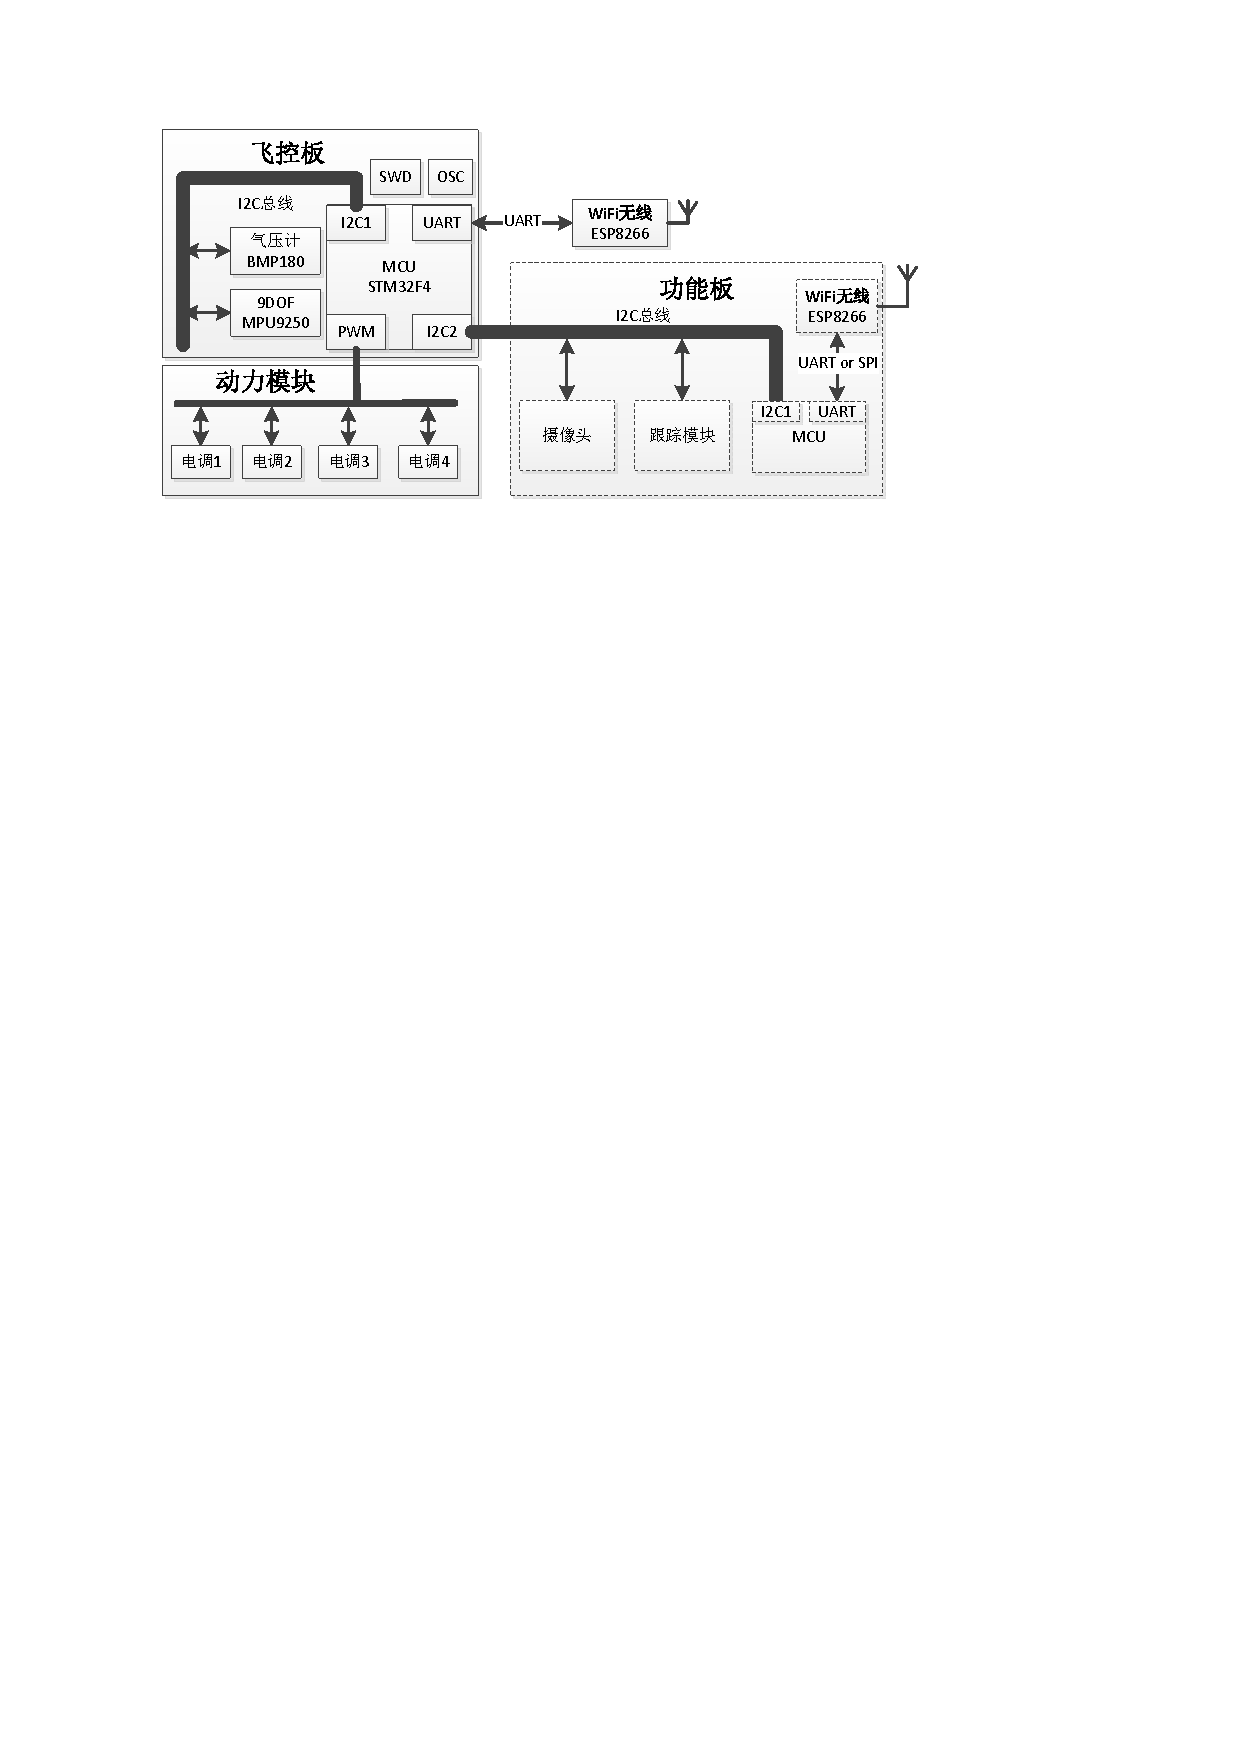
\includegraphics[width=12cm]{../fig/飞控板框图.pdf}
        \caption{飞控板框图}\label{飞控板框图}
    \end{center}
\end{figure}

飞行器控制系统主要包括核心的飞控板,无线模块和动力模块.其中飞控板是控制系统的核心,姿态算法和控制算法运行在其中的MCU中,该MCU中运行该项目专有的RTOS,飞控板的I2C1接口与9轴传感器MPU9250和气压(测高)传感器BMP180连接实时采样飞行器姿态.飞控板使用四路PWM控制动力模块的电调完成飞行控制.为了适应调试和后期的控制扩展飞控板预留WIFI模块接口UART,用于与上位机通信.飞行器上加载的功能,例如摄像,定位等使用独立的功能板实现并通过I2C2接口与飞控板通信.

RTOS结构框图如图\ref{cmos框图}:
\begin{figure}[!hbp]
    \begin{center}
        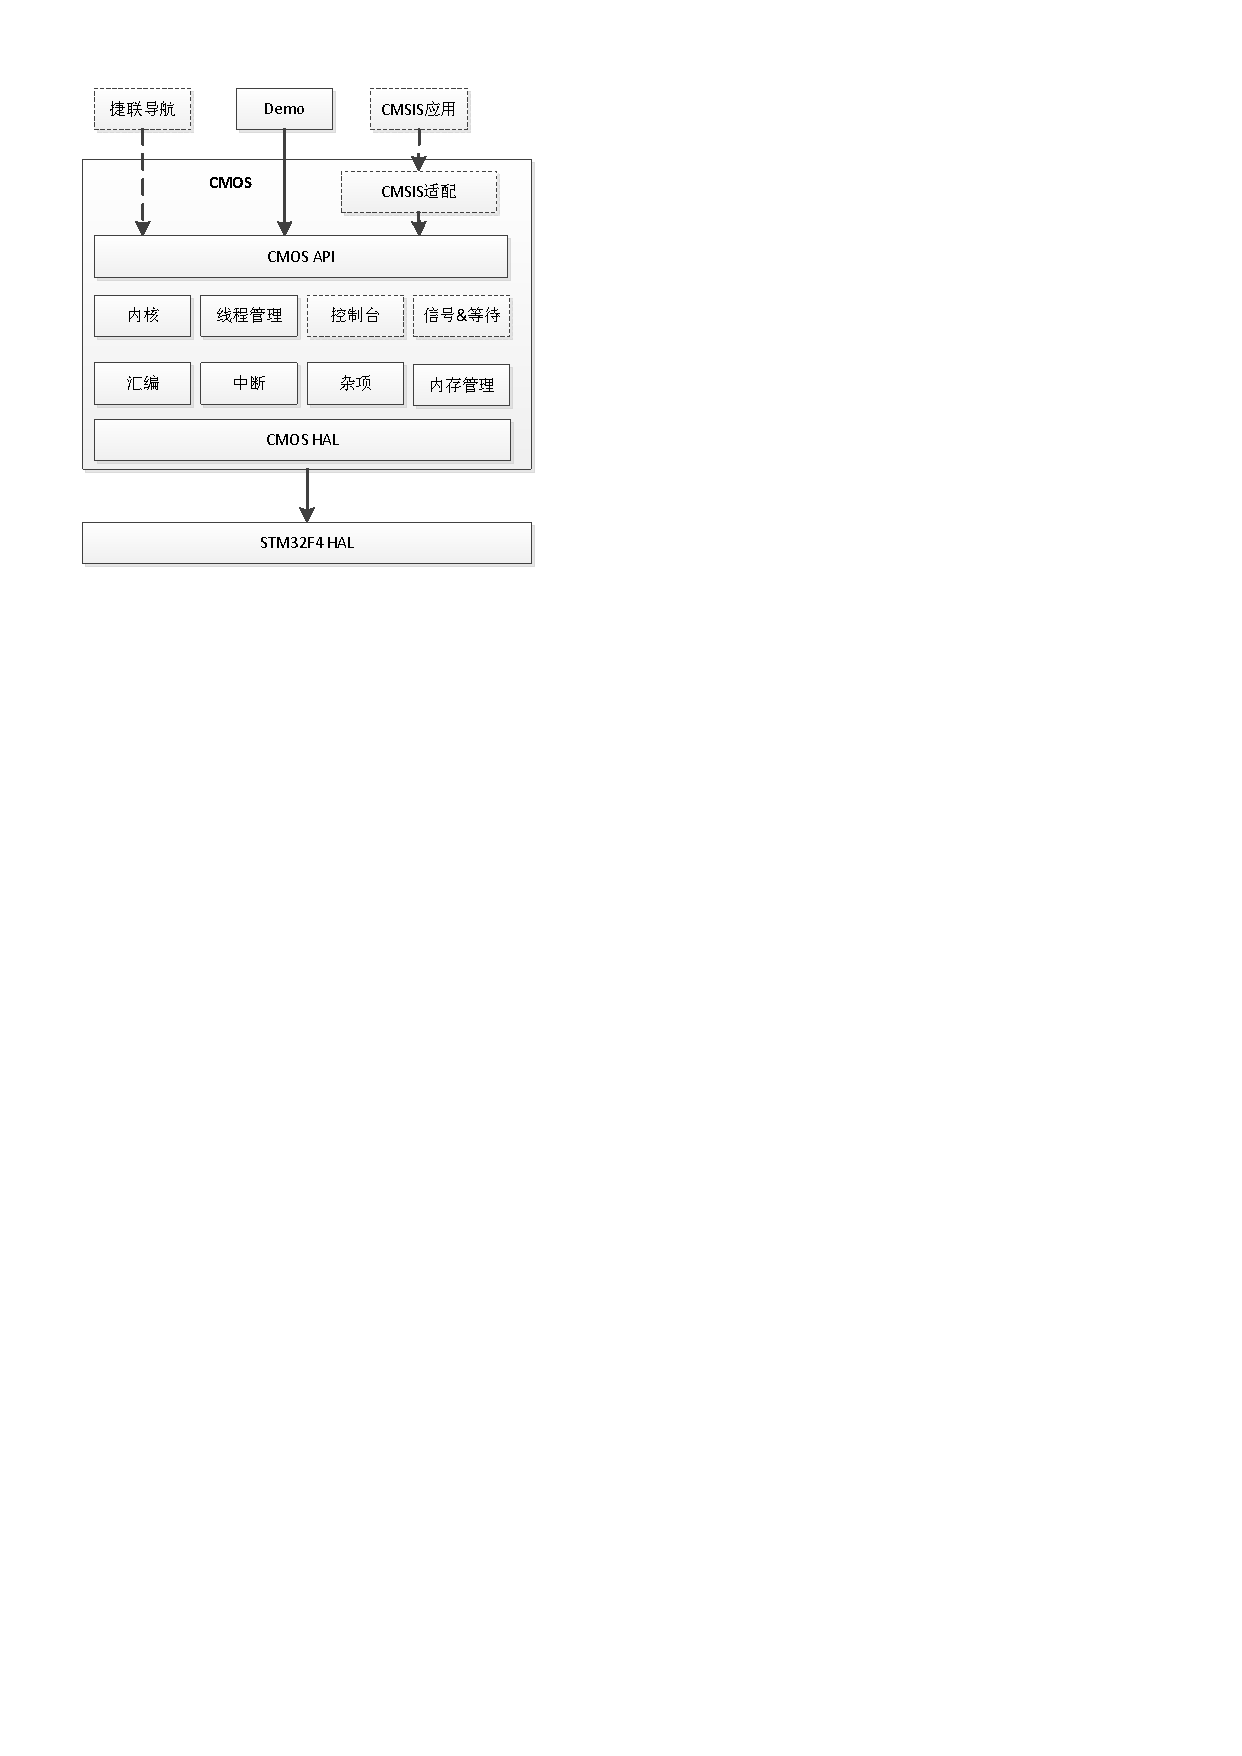
\includegraphics[height=12cm]{../../../../doc/CMOS结构框图.pdf}
        \caption{飞控板框图}\label{cmos框图}
    \end{center}
\end{figure}
图中,最底层由MCU厂商意法半导体提供,基于底层的硬件驱动RTOS做自己的适配层,基于适配层完成RTOS各模块的开发.

四轴飞行器中姿态角的求解算法在四轴飞行器设计中是核心内容,他完成飞行器自身姿态的计算,控制算法使用姿态计算出需要施加的控制量完成姿态控制.姿态算法的核心器件是陀螺仪,陀螺仪可以测量自身旋转的角速度.理论上只要陀螺仪精度足够,结合初始姿态通过积分可以计算飞行器任意时刻的姿态.然而,由于成本和尺寸的限制,四轴飞行器只能使用MEMS陀螺仪.MEMS陀螺仪精度不佳并有较大的漂移,在长时间的积分过程中会导致很大的积分误差,导致估计姿态随着时间累计而变得不可接受.为了解决这个问题,联想轮船,陀螺仪类似舵手,舵手长时间独立工作后会将船带偏,这个时候需要了望手来不断纠偏.通常四轴飞行器中使用加速度计来充当了望手,纠偏轮船的方向.加速度计通过测量重力场的方向纠正陀螺仪积分得到的姿态,普通的四轴飞行器使用陀螺仪和加速度计就可以完成精度可接受的姿态解算.但是,重力场方向竖直向下,可以纠正飞行器的水平倾斜,但飞行器绕重力场方向的旋转没法纠正。所以仅用6轴(陀螺仪3轴,加速度计3轴)融合的姿态只能保证飞行器的水平平衡,无法保证其航向稳定\footnote{会水平旋转},说通俗一点也就是飞行器会找不到北.类似加速度计的思路,传感器组合中加入一个测量地磁的传感器,就可以纠正飞行器航向上的偏移,这就是本文通所采用的9轴姿态融合.

姿态融合算法如图\ref{算法流程}:
\begin{figure}[!hbp]
    \begin{center}
        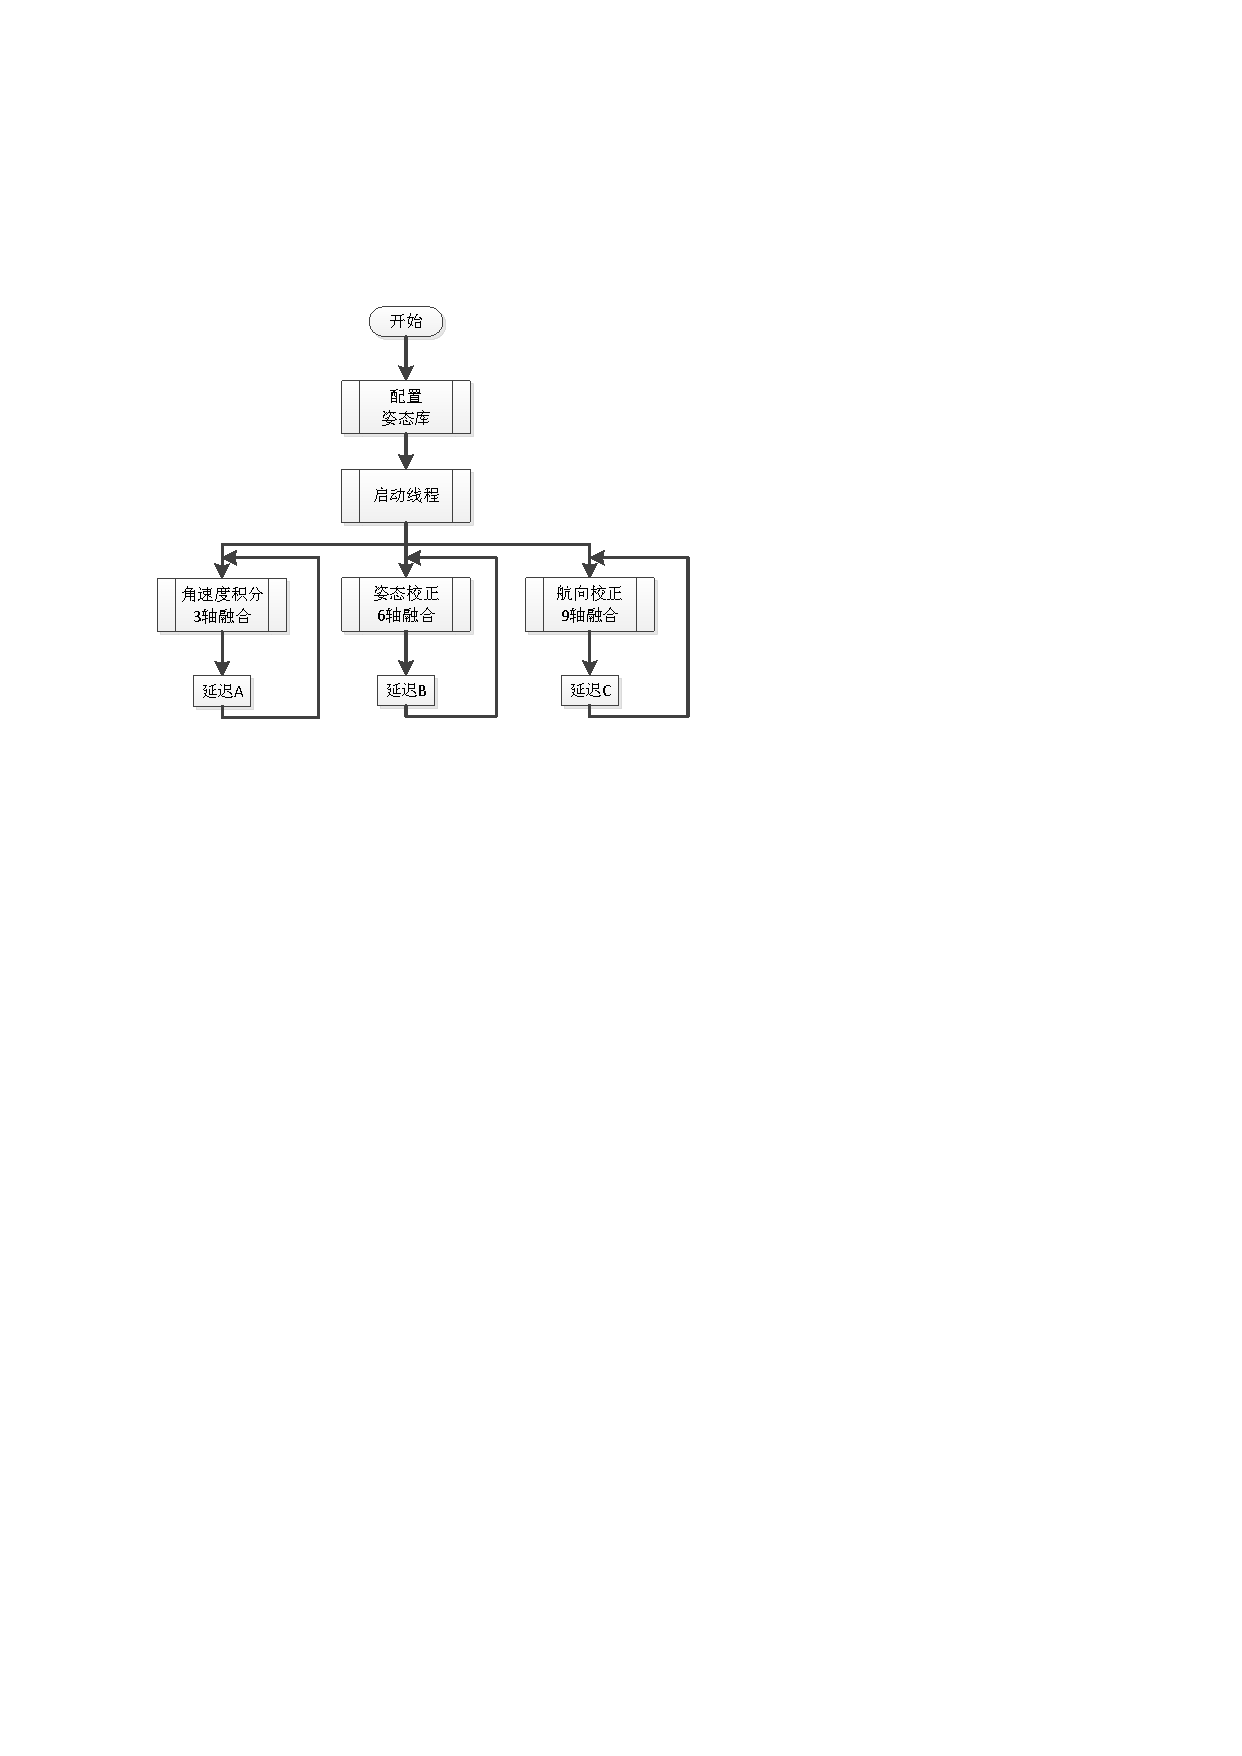
\includegraphics[height=10cm]{../fig/算法流程.pdf}
        \caption{算法流程}\label{算法流程}
    \end{center}
\end{figure}

\section{项目计划}
该项目的初步计划如表\ref{计划表}:
\begin{table}[!hbp]
\begin{center}
    \begin{tabular}{|l|l|}
        \hline
        工作内容 & 时间范围 \\ 
        \hline
        项目现状调研 & 2015.10.1至2015.12.1 \\
        \hline
        算法分析与调研 & 2015.12.1至2016.2.1 \\
        \hline
        CM3核RTOS调度算法 & 2016.2.1至2016.3.1 \\ 
        \hline
        飞控板设计与制作 & 2016.3.1至2016.5.1 \\
        \hline
        机框,电池,电调,螺旋浆选型采购 & 2016.5.1至2016.6.1 \\
        \hline
        姿态及控制算法的实现 & 2016.6.1至2016.8.1 \\
        \hline
        上位机软件设计 & 2016.8.1至2016.9.1 \\
        \hline
        整机联调与参数优化 & 2016.10.1至2017.1.1 \\
        \hline
\end{tabular}\caption{计划表\label{计划表}}
\end{center}
\end{table}

\section{成果与展望} 
项目成果成列与表\ref{成果表}:
\begin{table}[!hbp]
\begin{center}
    \begin{tabular}{|l|l|}
        \hline
        成果 & 表现形式 \\
        \hline
        飞行器样机食物 & 1套 \\
        \hline
        飞行器样机固件 & 1份(bin) \\
        \hline
        Android上位机APP & 1份(apk) \\
        \hline
        PC上位机PyQt & 1份(exe) \\
        \hline
        姿态融合算法核心期刊论文 & 1篇 \\
        \hline
        飞行器RTOS期刊论文 & 1篇 \\
        \hline
        飞行器整体结构论文 & 1篇 \\
        \hline
    \end{tabular}\caption{成果表\label{成果表}}
\end{center}
\end{table}

最后成型的样机实物图类似与图\ref{实物}:
\begin{figure}[!hbp]
    \begin{center}
        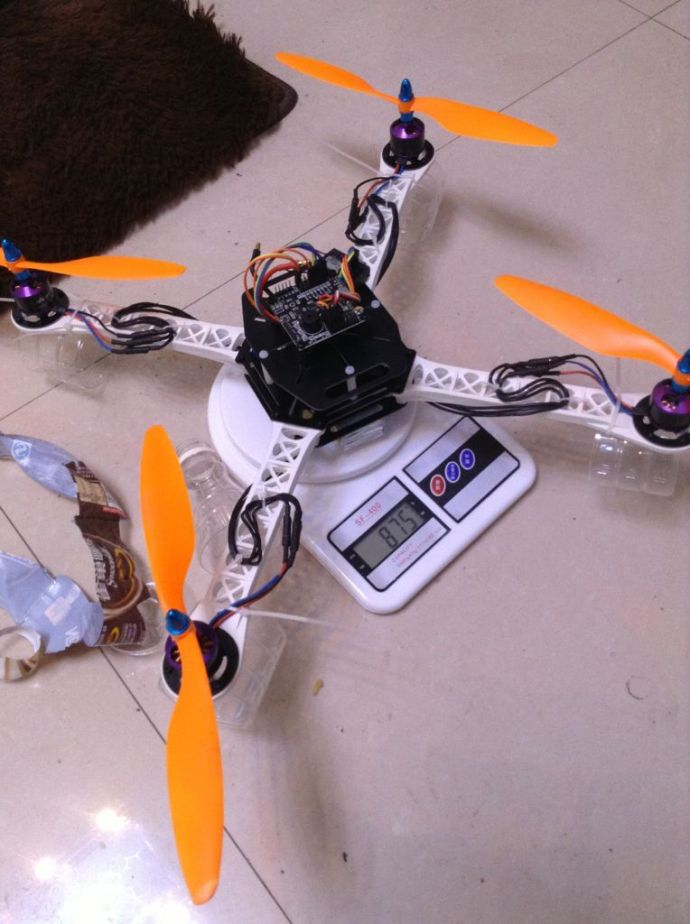
\includegraphics[height=5cm]{实物.jpg}
        \caption{实物}\label{实物}
    \end{center}
\end{figure}
后期展望,飞行器作为载体可以自主稳定飞行后可以加上功能板完成相应功能,例如自动跟踪,摄影,监控等.

% 参考文献
\newpage
% 将参考文献标题改为中文
% article 使用
\renewcommand\refname{参考文献}
% book 使用
\centering %居中
\bibliographystyle{plain}
\bibliography{main}

\end{document}

